\chapter{Elliptische Kurven über den komplexen Zahlen}

Nachdem wir elliptischen Kurven mittels einer Weierstrass-Gleichung
definiert haben, beschäftigen wir uns in diesem Kapitel über den
Spezialfall des Grundkörpers $K=\IC$. Hier gibt es einen Zugang zu
elliptischen Kurven über komplexe Analysis und Gitter in $\IC$. Einen
detailierten Zugang zu diesen Überlegungen ist in Kapitel VI von
Silvermans Buch~\cite{Silverman:AEC} zu finden. 

\begin{definition}
  Ein \emph{Gitter in $\IC$}\index{Gitter in $\IC$}, ist eine
  Teilmenge
  $$\Omega = \{\lambda_1 \omega_1 + \lambda_2 \omega_2 :
  \lambda_1,\lambda_2\in\IZ\}$$
  wobei $\omega_1,\omega_2\in\IC$ nicht auf einer Gerade
  durch den Nullpunkt liegen. 
\end{definition}

Die Bedingung an $\omega_1,\omega_2$ schliesst aus, dass
$\omega_1\omega_2=0$ und dass es $\lambda\in\IR$ gibt, so dass
$\omega_1 = \lambda\omega_2$.

\begin{aufgabe}
  Zeigen Sie, dass $\omega_1,\omega_2\in\IC$ genau dann auf einer
  Gerade durch den Nullpunkt liegen, wenn
  \begin{equation*}
    \det \left(
      \begin{array}{ll}
        \omega_1 & \omega_2 \\
        \overline{\omega_1} & \overline{\omega_2}
      \end{array}
    \right)=0,
  \end{equation*}
  dabei bezeichnet $\overline{\cdot}$ komplexe Konjugation. 
\end{aufgabe}

Ein Gitter $\Omega\subset\IC$ ist abgeschlossen unter der Addition auf
$\IC$ und unter Multiplikation mit $-1$. Es ist eine Untergruppe der
additive Gruppe des Körpers $\IC$.

Das Paar $(\omega_1,\omega_2)$ nennt man auch Basis des Gitters
$\Omega$. Kurzhand Notation ist $\Omega = \omega_1\IZ +\omega_2\IZ$.
Die Basis ist \underline{nicht} eindeutig durch das Gitter festgelegt.


\begin{beispiel}
  Das Gitter mit Basis $(1,e^{2\pi
    \sqrt{-1}/6})$
  ist in Abbildung
  \ref{fig:lattice} darsgestellt. 
  \begin{figure}
    \centering    
    \caption{Das Gitter $\IZ+\omega\IZ$ mit $\omega = e^{2\pi\sqrt{-1}/6}$}
    \label{fig:lattice}
    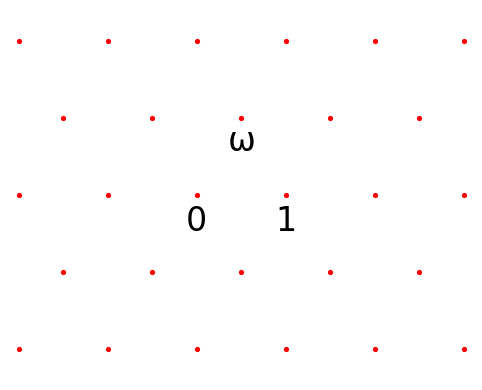
\includegraphics[width=0.3\textwidth]{./plots/lattice.png}
  \end{figure}
\end{beispiel}

Gegeben sei ein Gitter $\Omega$, wir können dazu eine Funktion
konstruieren. Für $z\in \IC\ssm\Omega$ definieren wir
\begin{equation}
  \label{def:wp}
  \wp_\Omega(z) = \frac{1}{z^2} + \sum_{\omega\in \Omega\ssm\{0\}}
  \left(\frac{1}{(z-\omega)^2} - \frac{1}{\omega^2}\right).
\end{equation}

\begin{bemerkung}
  Die Reihe (\ref{def:wp}) konvergiert absolut für alle
  $z\in\IC\ssm\Omega$.
  Für $\omega\not=0$ und
  $\omega\not=z$ ist der
  Absolutbetrag von 
  \begin{equation*}
    \frac{1}{(z-\omega)^2} - \frac{1}{\omega^2} =
    \frac{\omega^2 - (z-\omega)^2}{(z-\omega)^2\omega^2}
    =\frac{-z^2 + 2z\omega}{(z-\omega)^2\omega^2}
  \end{equation*}
  höchstens $C(z)/|\omega|^3$, wobei $C(z)>0$ von $\omega$ unabhängig
  ist. 
\end{bemerkung}

Ohne Beweis halten wir die folgenden Fakten fest.
Die Abbildung $z\mapsto \wp_\Omega(z)$ ist wohldefiniert und komplex
differenzierbar auf $\IC\ssm\Omega$. Sie ist eine meromorphic Funktion
mit einer doppelten Polstelle an jedem Punkt auf $\Omega$. 
Man nennt $\wp_\Omega$ die \emph{Weierstrass-$\wp$
  Funktion}\index{Weierstrass-$\wp$ Funktion}.

\begin{lemma}
  Sei $\Omega \subset\IC$ eine Gitter und $\wp_\Omega$ die Funktion
  oben. Für alle $z\in\IC\ssm\Omega$ erfüllt die Ableitung
  \begin{equation}
    \label{eq:wpderiv}
    \wp_\Omega'(z) = -2 \sum_{\omega\in\Omega} \frac{1}{(z-\omega)^3}.
  \end{equation}
  Für alle $z\in\IC\ssm\Omega$ und alle  $\omega\in\Omega$
  gilt $\wp_\Omega(z+\omega) = \wp_\Omega(z)$ und
  $\wp'_\Omega(z+\omega) = \wp'_\Omega(z)$.
\end{lemma}
\begin{proof}
  Die Formel für die Ableitung folgt aus (\ref{def:wp}), man darf
  summandenweise Ableitung, da die Reihe absolut konvergiert. Es gilt
  $\wp'_\Omega(z+\omega) = \wp'_\Omega(z)$ wie im zweiten Teil der
  Aussage, da die Summe (\ref{eq:wpderiv}) invariant unter Translation
  von $z$ um ein Gitterpunkt ist.
  Es folgt damit
  $$
  \wp_\Omega(z+\omega) = \wp_\Omega(z) + c(\omega)
  $$
  wobei $c(\omega)$ nur von $\omega$ aber nicht von $z$ abhängt.
  Wir setzen $z=-\omega/2$ ein und finden
  $\wp_\Omega(\omega/2) = \wp_\Omega(-\omega/2) + c(\omega)$.
  Aber man kann sich aus (\ref{def:wp}) davon überzeugen, dass
  $\wp_\omega(z)=\wp_\omega(-z)$ gilt, d.h. $\wp_\omega$ ist eine
  gerade Funktion. Es folgt $c(\omega)=0$. 
\end{proof}

\begin{bemerkung}
  Sowohl $\wp_\Omega$ wie auch $\wp'_\Omega$ sind \emph{doppelperiodische
    Funktionen}. Deshalb werden die Elemente aus $\Omega$ auch
  Perioden genannt. 
\end{bemerkung}

Ohne Beweis erwähnen wir, dass $\wp_\Omega$ eine wichtige
Differentialgleichung erfüllt. Genauer, es gibt $g_2,g_3\in\IC$, so
dass
\begin{equation}
  \label{eq:discg2g3}
  g_2^3-27g_3^2 \not=0
\end{equation}
und 
\begin{equation}
  \label{eq:weierstrassdgl}
  {\wp_\Omega'}^2  = 4 \wp_\Omega^3 - g_2\wp_\Omega - g_3.  
\end{equation}


Bis auf den Faktor $4$ liegen die Werte des Paars
$(\wp_\Omega,\wp'_\Omega)$ auf einer elliptischen Kurve. 
Die Bedingung (\ref{eq:discg2g3}) entspricht dabei der Bedingung
(\ref{eq:disccondition}).

Der Faktor $4$ ist harmlos, wir können die gesamten Überlegungen aus
Kapitel~\ref{kap:ek} auf die \emph{modifizierte Weierstrass-Gleichung}
\begin{equation}
  \label{eq:modweierstrass}
  Y^2 = 4X^3-g_2X-g_3 \quad\text{wobei}\quad   g_2^3-27g_3^2 \not=0
\end{equation}
anwenden und ein Gruppengesetzt auf $E(\IC)$ definieren.

Wir definieren eine Abbildung
\begin{alignat*}1
  \Psi \colon &\IC\rightarrow E(\IC)
\end{alignat*}
durch
\begin{equation*}
  \Psi(z) = \left\{
    \begin{array}{ll}
      (\wp_\Omega(z),\wp'_\Omega(z)) &: z\not\in\Omega, \\
      \cO &:z\in \Omega.
    \end{array}\right.
\end{equation*}

Wegen der Doppelperiodizität von $\wp_\Omega$ und $\wp'_\Omega$
gilt $\Psi(z+\omega) = \Psi(z)$ für alle $z\in\IC$ und alle
$\omega\in\Omega$.

Weiterhin, und dies ist nicht trivial, ist $\Psi$ ein
Gruppenhomomorphism, wobei wir $\IC$ als additive Gruppe des Körpers
der komplexen Zahlen verstehen. Schliesslich ist $\Psi$ auch eine
surjektive Abbildung. Aus diesen Überlegungen folgt, dass
\begin{equation*}
  \IC/\Omega \quq E(\IC)\quad\text{vermöge $\Psi$ als Gruppen isomorph sind.}
\end{equation*}

Weiterhin können trägt $E(\IC)$ wegen der Interpretation aus Abschnitt
\ref{sec:projektiv} die Struktur eines topologischen Raums.
Aus
topologischer Sicht sind $\IC/\Omega$ und $E(\IC)$ ununterscheidbar.

\begin{bemerkung}
  Aus topologischer Sicht ist $\IC/\Omega$ nichts anderes als ein
  Torus, vgl. Abbildung~\ref{fig:torus}.
    \begin{figure}
      \centering
      \caption{Ein Torus}
    \label{fig:torus}
    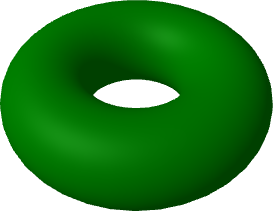
\includegraphics[width=0.3\textwidth]{./plots/torus.png}
  \end{figure}
  Topologisch gesehen sehen alle elliptischen Kurven über $\IC$ gleich
  aus. Aber die elliptische Kurve selber trägt zusätzliche Struktur,
  da sie schlussendlich von einer Weierstrass-Gleichung kommt. Diese
  Struktur ist für die Topologie ``unsichtbar'', aber nicht für die
  komplexe Geometrie. 
\end{bemerkung}

Eine modifizierte Weierstrass-Gleichung (\ref{eq:modweierstrass}) legt
ein Gitter $\Omega\subset\IC$ fest, für welches
(\ref{eq:weierstrassdgl}) gilt.  Die ``Perioden'' in $\Omega$ lassen
sich durch  Integrale
\begin{equation*}
  \int \frac{dx}{\sqrt{4x^3-g_2 x - g_3}}
\end{equation*}
bestimmen. Das Integral findet auf bestimmten Schleifen  in $\IC$ statt
und der Wert des Integrals hängt auch von der Schleife ab.  Diese
Integrale heissen aus historischen Gründen \emph{elliptischen
  Integrale} und sind verantwortlich für den Begriff ``elliptisch'' in
elliptische Kurve.\footnote{Elliptische Kurven sind keine Ellipsen!}

%%% Local Variables:
%%% TeX-master: "main"
%%% End:

